\documentclass[conference]{IEEEtran}
\IEEEoverridecommandlockouts
% The preceding line is only needed to identify funding in the first footnote. If that is unneeded, please comment it out.
\usepackage{cite}
\usepackage{amsmath,amssymb,amsfonts}
\usepackage{algorithmic}
\usepackage{hyperref}
\usepackage{graphicx}
\usepackage{textcomp}
\usepackage[ruled,vlined]{algorithm2e}
\usepackage{listings}
\usepackage{xcolor}
\usepackage{etoolbox}
\usepackage{fancyhdr}
\lstset { %
    language=C++,
    backgroundcolor=\color{black!5}, 
    basicstyle=\footnotesize,
}
\makeatletter
\patchcmd{\@makecaption}
  {\scshape}
  {}
  {}
  {}
\makeatletter
\patchcmd{\@makecaption}
  {\\}
  {:\ }
  {}
  {}
\def\footnoterule{\kern-3\p@
  \hrule \@width 3.5in \kern 2.6\p@}
\makeatother
\def\tablename{Table}
\def\BibTeX{{\rm B\kern-.05em{\sc i\kern-.025em b}\kern-.08em
    T\kern-.1667em\lower.7ex\hbox{E}\kern-.125emX}}
\pagestyle{fancy}
\fancyhf{}
\rfoot{Mentor: Prof. Jayprakash Lalchandani}
\begin{document}
\title{Slicing Shared Memory Parallel Programs\\
}

\author{\IEEEauthorblockN{1\textsuperscript{st} Rahul Purohit}
\IEEEauthorblockA{\textit{Information and Communication Technology (minors in CS)} \\
\textit{DA-IICT}\\
Gandhinagar, India \\
201701161@daiict.ac.in}
\and
\IEEEauthorblockN{2\textsuperscript{nd} Harshil Patel}
\IEEEauthorblockA{\textit{Information and Communication Technology} \\
\textit{DA-IICT}\\
Gandhinagar, India \\
201701177@daiict.ac.in}
}

\maketitle

\begin{abstract}
Program slice of a program is defined such that all the program statements that potentially might affect the variable of interest. Program slicing has many applications ranging from software testing, software debugging, understanding and maintainability  of a program, etc. 
\par OpenMP is an application programming interface which allows an user to develop shared memory parallel programs. It has many constructs which affect the program such that the program can be executed on a multiprocessor workstation. 
\par This project aims at analyzing the parallel and concurrent program (made using a shared memory programming construct like OpenMP) using different Slicing techniques like  and develop a tool using which an user can obtain program slices of C++ programs written with OpenMP.
\end{abstract}

\begin{IEEEkeywords}
program slicing, shared memory parallel programs, static slicing, dynamic slicing, program dependencies
\end{IEEEkeywords}

\section{Introduction}
As mentioned earlier, Program Slicing is related with all the statements that might be affected (or potentially affected) by the different statements\cite{b1}. It might even depend on the given input to the program. If the program slice is obtained keeping in mind the input, then such program slicing technique is called dynamic program slicing, on the other side if the program slice is obtained without any input but keeping in mind all the possibilities the program might get executed then it is static program slicing. Now there are many methods, using which we can obtain static or dynamic program slices, but the inherent methods might be using graph techniques or may be using different data structures using which we can obtain the program slice.
\par Any program slice is defined in terms of it's slicing criterion. Slicing criterion $SC= < L , V , I >$, where $L$ is the part of the program whose slice we want to find(generally the line number), $V$ is the variable or set of variables, whose program slice we are interested in and $I$ which is only in the case of a dynamic technique, is the given input for the program.
\par OpenMP is can be used as an API which can be used to develop programs that can leverage the multi-processor system and all the memory components of the  workstation. Finding the program slice in some methods does require the trace of the execution of the program. The programs that are ran on threads depending on the different methods, workstations and the logic used, the resultant execution trace $EH$ of the program can be very different from the trace of a normal sequential program. So OpenMP programs take into account local properties of the workstation on which the program is being executed, so there can be different programs that might give the optimal parallelization on different workstations. Thus the need of a tool that can give insight to such programs becomes further important.   
\par There are many different slicing techniques for static and dynamic slicing methods, but we would focus on 4 methods and try to develop the algorithms for them by making changes to the existing algorithms. The methods would be for each of the following: $(i)$ Static Graph-less slicing method, $(ii)$ Static Graph-based slicing method, $(iii)$ Dynamic Graph-less slicing method and $(iv)$ Dynamic Graph-based slicing method.

\section{Design}
\subsection{User Stories}
Before Developing the tool or implementing any algorithms the user stories would be an important part using which the goal of the development of the tool would be achieved. The main user stories upon which this project focuses on are as follows:
\begin{figure*}[t]
    \centering
    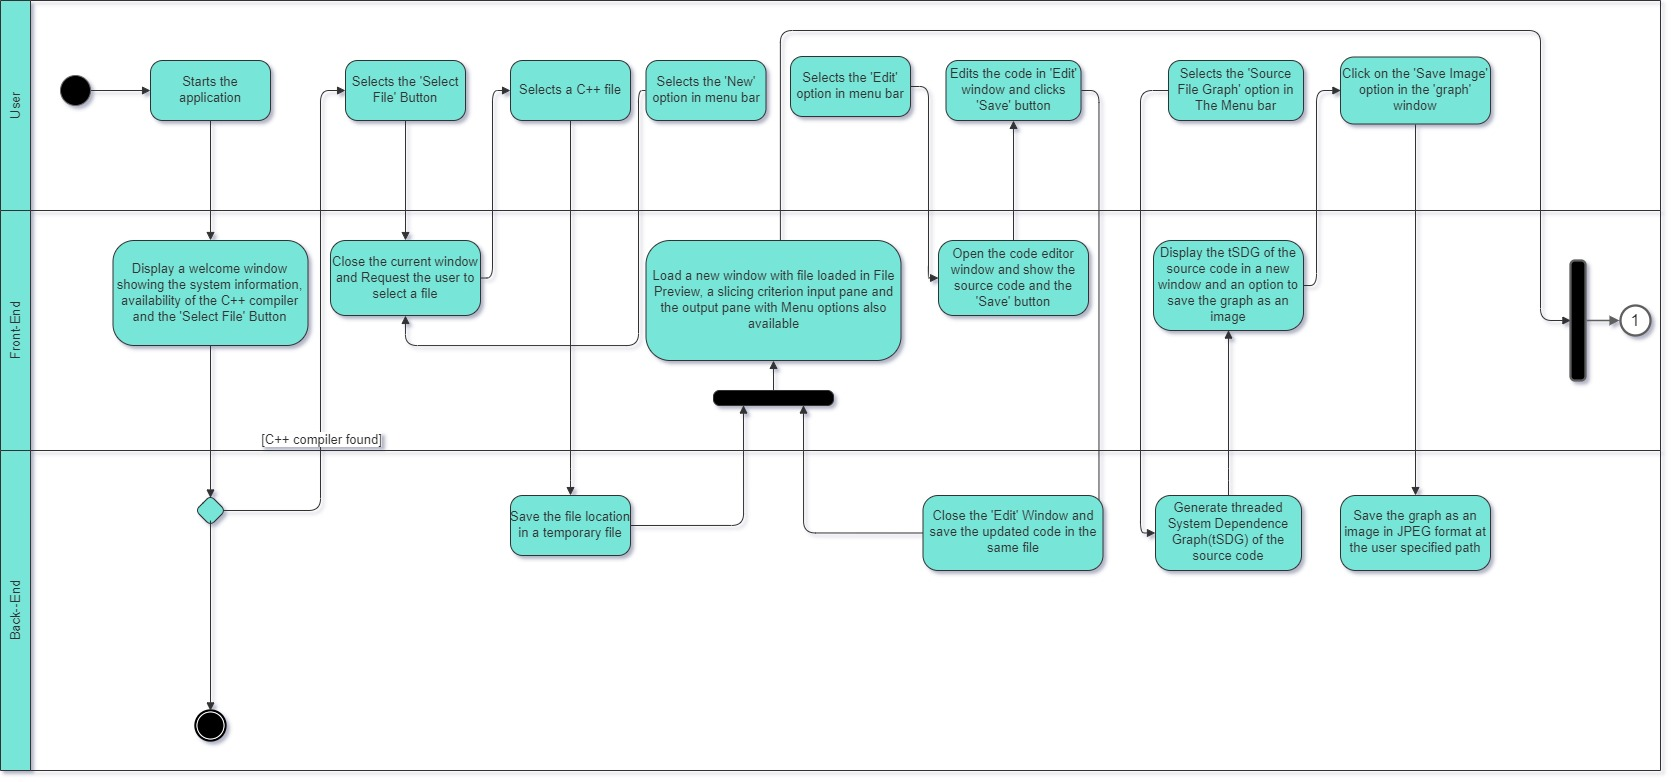
\includegraphics[scale=0.3]{UML_Activity_Left.jpg}
    \caption{UML activity diagram Part 1}
    \label{fig:my_label}
\end{figure*}
\begin{figure*}[t]
    \centering
    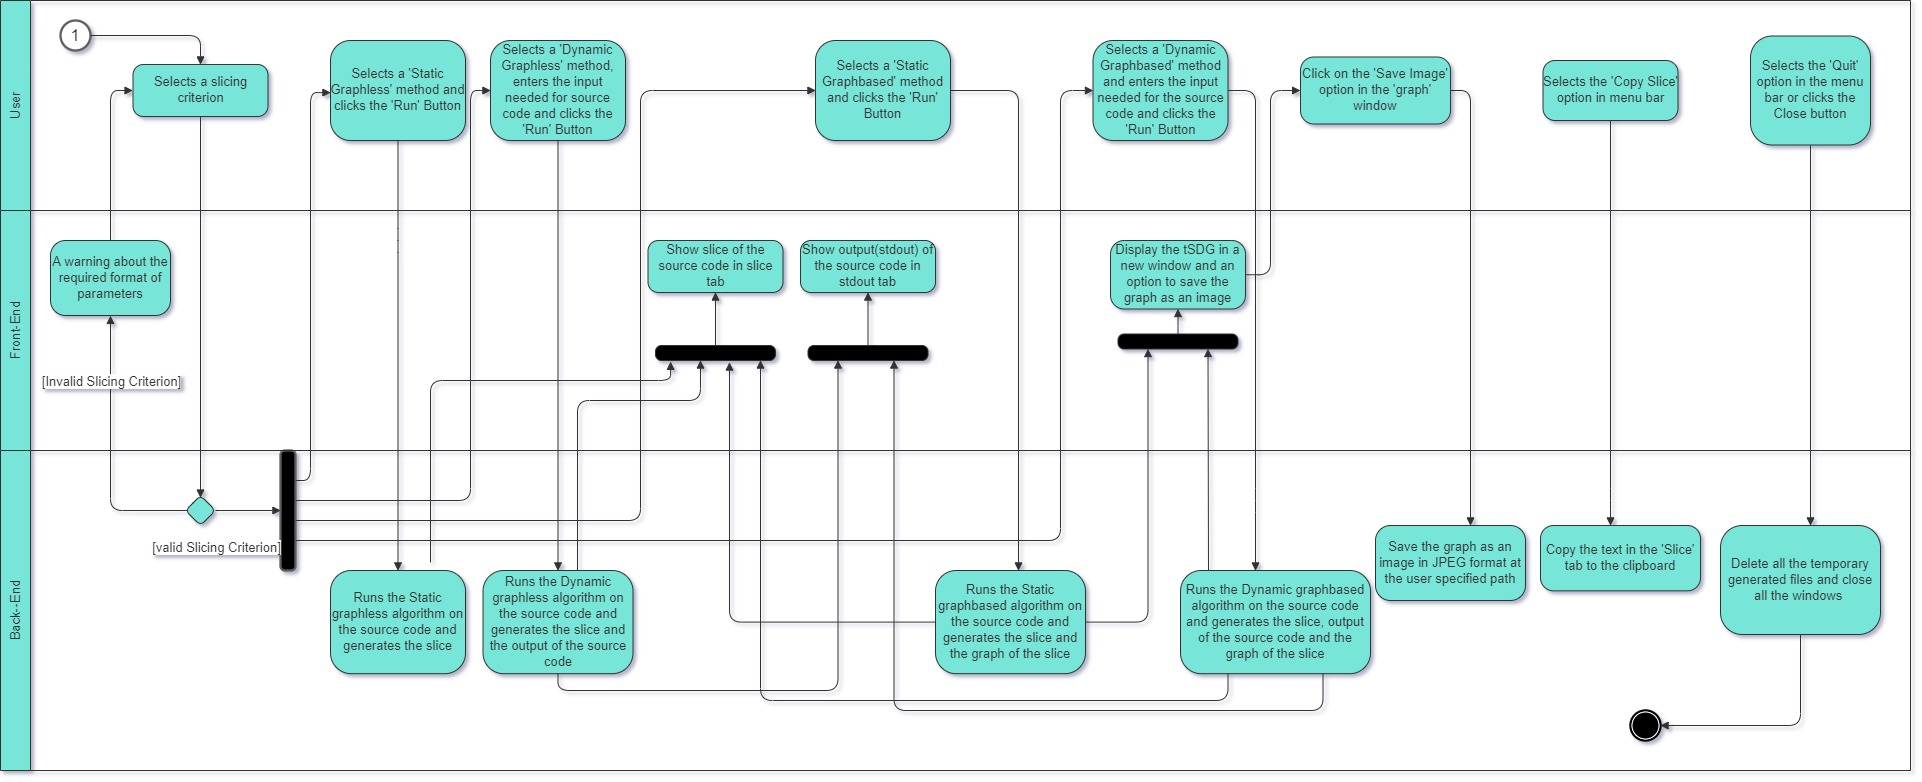
\includegraphics[scale=0.27]{UML_Activity_Right.jpg}
    \caption{UML activity diagram Part 2}
    \label{fig:my_label}
\end{figure*}
\begin{itemize}
    \item As a Programmer/Debugger/Software Maintainer, I want to see the program slice of a C++ program, so that I can find the dependencies a particular variable has in whole of the program and debug the program (if necessary).
    \item As a Programmer/Debugger/Software Maintainer, I want to be able to get a graphical representation of the slice, so that I can visualize the program slice with the dependencies between the nodes(lines) in the graph.
    \item As a Programmer/Debugger/Software Maintainer, I want to be able to have a tool that can take my C++ code with the OpenMP construct with a particular input and give me the dynamic program slice, so that I can find the dependencies in the code pertaining to the input.
    \item As a Programmer/Debugger/Software Maintainer, I want to be able to save a graph as an image, so that I can share and use it anywhere else in the future.
    \item As a Programmer/Debugger/Software Maintainer, I want to be able to edit the source code, so that I can add or delete the lines if needed.
    \item As a Programmer/Debugger/Software Maintainer, I want to be able to copy the generated slice in the clipboard, so that I can paste it wherever I want.
    \item As a Programmer/Debugger/Software Maintainer, I want to be able to see the tSDG of the whole source code, so that I can compare it with the graph of the slice.
\end{itemize}
\subsection{Activity Diagram}
Designing a tool, would also require how the tool would interact with the user. So $Fig. 1$ is the activity diagram of the interaction between the tool and the user and how the user can get the needed program slice and all the other things the user would like to use. The three swim-lanes shows the major parts of the application and how they would interact, namely user, front-end with which user interacts and the back-end which would execute all the requests.

% \subsection{GUI Design}
% A window image

\section{Implementation}
\par The goal of this project is to develop a tool which helps an user to interact with it and asks them for a C++ code with OpenMP constructs and the Slicing criteria $SC$. There would be four different methods that would be available to help find the program slice.
\subsection{Technologies Used and the Supported Constructs}
\par All the four algorithms (namely Static Graph Based Program Slicing, Static Graph-less Program Slicing, Dynamic Graph Based Program Slicing and Dynamic Graph-less Program Slicing) were written using \textbf{C++} and the target programs are programs that are written using \textbf{OpenMP}\footnote{Please refer to the Appendix Section A,B and C for more information on the OpenMP constructs and what are their features.} constructs. The reason to select C++ for writing algorithms was due to the performance factor and also the flexibility C++ provides in respect to the handling of data structures. One more advantage that we can obtain is the way user can directly interact with the algorithms written in C++ and obtain the desired data structures and output.
\begin{table}[h!]
\begin{center}
\begin{tabular}{| p{0.12\textwidth} | p{0.27\textwidth} |}
\hline
    \textbf{Parallel Control constructs} & PARALLEL, FOR, SECTION, SINGLE, MASTER  \\
\hline
    \textbf{Data constructs} & PRIVATE, SHARED, THREADPRIVATE, REDUCTION  \\
\hline
    \textbf{Synchronization} & BARRIER, FLUSH, CRITICAL  \\
\hline
\end{tabular}
\end{center}
\caption{Supported OpenMP Constructs}
\label{tab:template}
\end{table}
% \subsection{GUI Application Construction}
\par The GUI application is made using the Tkinter library of \textbf{Python 3}. The application also uses other libraries namely os, shutil and subprocess (Interacting with the file system), pydot, graphviz and networkx (for visualizing and drawing graphs) for various processes. The GUI application needs the Algorithm in the same folder so that it can function properly. The reason to choose Python for the front-end was due to the need of a lightweight GUI application and Tkinter would provide us with those basic functionalities and also It provides with the important file handling and system command libraries along with the advanced graph making libraries which would be needed to realise the graphs in the case of the Graph based slicing approaches. Another important reason to develop an application which works locally was due to the reason of OpenMP applications. These applications need to be tested in the local environment rather than a remote server, whose properties might be different. 
\subsection{Parser}
\par In these algorithms we have used our own parser, because currently we have handled basic and frequent keywords used in the C++ OpenMP programs.A. Beszedes et al.\cite{b2} presented a possible way to parse C programs, our parser took the inspiration from them but the difference being in the difference of environment. So using our parser in place of existing one reduces memory usage. Basically what out parser does is it process the whole source code line by line. It takes the line and finds the token exists on that line and depending upon different token which matches with the C++(given below) and OpenMP constructs(shown in $Table$ $1$) it processes it accordingly. 
\subsubsubsection{C++ Constructs}
\begin{itemize}
\item I/O Statements like $cin,cout$
\item Built-In Data-types like $int, float, double, string, void$
\item Conditional Statements like $if-else$
\item Loop Constructs like $for, while$
\item Function Declarations and Function Definitions
\item Comments of type $"//"$
\item Handling user defined header files like $#include$
\item Calling functions from different header files
\item Handling library functions
\item Definition Statements like $a = b + c$\\
\end{itemize}
\subsection{Algorithm}
\par In the calculation of graph-less algorithm we have used global algorithm for backward slicing approach presented by A. Beszedes $et$ $al.$\cite{b3}, the algorithm tries to maintain a $D/U$ representation of program, $i.e.$, defined variables and used variables at each program line, using the execution history $EH$, which can be calculated for both static and dynamic cases.  
\begin{algorithm}[h]
 \caption{Dynamic Backward Graph-less Slicer}
 \begin{algorithmic}[1]
 \renewcommand{\algorithmicrequire}{\textbf{Input:}}
 \renewcommand{\algorithmicensure}{\textbf{Output:}}
 \REQUIRE $P$ : a program\\
  x : a program input
 \ENSURE  backward slices for all (x, J, V) criteria\\$(j = 1...J,V_j = U(j))$\\
  \STATE {Read $EH$}
  \FOR {$j \gets 1$ to $J$}
    \STATE {$line$ $\gets$ $P(EH(j))$}\\
    \STATE {$d(j)$ $\gets$ {process(line)}}\\
    \STATE {$DynDep(d(j)) $ $\gets$ $\cup_{u_k\in U(j)}${($DynDep(u_k)\cup$ \\ {$LS(u_k)$}) }}\\
    \STATE {$LS(d(j))  $ $\gets$ {$j$}}\\
  \ENDFOR
  
 \RETURN $DynDep(V)$ as the backward dynamic slice\\ for the criterion $(x, J, V) $
 \end{algorithmic}
 \end{algorithm}
 \par Now, the basic idea of the algorithm is that for the requested slicing criteria, to find the slice $DynDep(V)$, where $V$ is the variable, we would start processing the lines before the line number whose slice is requested and till the line number where the slice is requested, for each line we would try to find for all the used variables $u_{line}$ at the line, their last defined line number $LS(u_{line})$, which would be the part of the slice. Hence, in this way we would calculate the slice from the $D/U$ representation which would also take in context the OpenMP constructs, which would be treated like control statements as variables that are defined on the line where they are first declared and all the corresponding lines of the control structure section would use that variable.
 \par Agarwal and Horgan, presented a dynamic slicing algorithm, which uses a graph\footnote{Please refer to Appendix Sections D, E, F, G and H for more information on different kind of graph representations.} to represent the program\cite{b4}. There are many papers that discuss graph based algorithms to represent the shared memory parallel programs\cite{b5}\cite{b6}. For a program for the graph-based algorithm we would need the representation of the program as a graph where the nodes are the program lines and the edges are the dependencies as can be seen from $Algorithm$ $2$, we have defined how edges are created in the implementation section.
 \begin{algorithm}[h!]
 \caption{Algorithm to Construct tSDG}
 \begin{algorithmic}[1]
 \renewcommand{\algorithmicrequire}{\textbf{Input:}}
 \renewcommand{\algorithmicensure}{\textbf{Output:}}
 \REQUIRE $P$ : a program\\
 \ENSURE  threaded System Dependence Graph for $P$\\
  \STATE {Parse the source code line by line and create different nodes for each line depending upon parsed keyword}\\
\STATE {In all these nodes store the variables which are defined and used on that line}\\
\STATE {Add $data\ dependence\ edge$ between the nodes where the variable is used to where the variable is last defined before the used variable’s line}\\
\STATE {Add $control\ dependence\ edge$ between the current node and its enclosing scope node}\\
\STATE {Add $Interference\ dependence\ edge$ between nodes where nodes are data dependent to each other but executed from different threads}\\
\STATE {Upon finding function definition create $formal-in\ nodes$ for all function parameters, $formal-out\ nodes$ for all function parameters which are passed by reference and $function\ node$
}\\
\STATE {Upon finding a call to the procedure create $call site\ node$, $actual-in\ nodes$ for all function arguments and $actual-out\ node$ for all function arguments which are passed by reference
}\\
\STATE {Add a $call\ edge$ from the call site node to the corresponding function node
}\\
\STATE {Add $parameter-in\ edge$ between actual-in node to its corresponding formal-in node for all actual-in node at call site}\\
\STATE {Add $parameter-out\ edge$ between formal-out node to its corresponding actual-out node for all formal-out node}\\
\STATE {$Transitive\ dependence\ edge$ is created from an actual-in node to an actual-out node if there exist intraslice-path from the formal-out node to formal-in node}\\
\STATE {$Affect-return\ edge$ is created from an actual-in node to the call site node if there exist intraslice-path from the formal-out node to formal-in node}\\
\STATE {For each return site in the called procedure $Q$, a $return-link\ edge$ is created from the return node in $Q$ to each call site that calls $Q$}\\
 \end{algorithmic}
 \end{algorithm}
  \begin{algorithm}[h!]
 \caption{Dynamic Backward Graph-based Slicer}
 \begin{algorithmic}[1]
 \renewcommand{\algorithmicrequire}{\textbf{Input:}}
 \renewcommand{\algorithmicensure}{\textbf{Output:}}
 \REQUIRE $G$ : tSDG of program\\
$x$ : a program input

 \ENSURE  backward slices for the criteria $(x, J, V)$\\
  \STATE {$// Phase 1$}\\
  \STATE {Queue queue $\gets$ V which belongs to line no. J}\\
  \WHILE{!queue.empty()}
    \STATE {curr $\gets$ queue.front()}\\
    \STATE {queue.pop();}\\
    \IF{ans.find(curr) == ans.end()}
        \STATE {ans $\gets$ curr}\\
    \ENDIF
    \STATE {queue $\gets$ curr$\rightarrow$parent}\\
    \STATE {queue $\gets$ curr$\rightarrow$interference\_edge}\\
    \STATE {queue $\gets$ curr$\rightarrow$parameter\_in\_edge}\\
    \STATE {queue $\gets$ curr$\rightarrow$calling\_edge}\\
    \STATE {queue $\gets$ curr$\rightarrow$transitive\_edge}\\
    \STATE {queue $\gets$ curr$\rightarrow$affect\_return\_edge}\\
  \ENDWHILE
  \STATE{}\\
  \STATE {$// Phase 2$}\\
  \STATE {queue $\gets$ ans}\\
  \WHILE{!queue.empty()}
    \STATE {curr $\gets$ queue.front()}\\
    \STATE {queue.pop()}\\
    \IF{ans.find(curr) == ans.end()}
        \STATE {ans $\gets$ curr}\\
    \ENDIF
    \STATE {queue $\gets$ curr$\rightarrow$parent }\\
    \STATE {queue $\gets$ curr$\rightarrow$interference\_edge}\\
    \STATE {queue $\gets$ curr$\rightarrow$parameter\_out\_edge}\\
    \STATE {queue $\gets$ curr$\rightarrow$transitive\_edge}\\
    \STATE {queue $\gets$ curr$\rightarrow$affect\_return\_edge}\\
    \STATE {queue $\gets$ curr$\rightarrow$return\_link\_edge}\\
  \ENDWHILE
  
 \RETURN $ans$ as the backward dynamic slice\\ for the criterion $(x, J, V) $
 \end{algorithmic}
 \end{algorithm}
 After obtaining the $tSDG$ for the program using the algorithm described in $Algorithm$ $2$, to calculate the program slice, the problem boils down to a graph-reachability problem, as described in $Algorithm$ $3$. To find the program slice for the slicing criteria, the algorithm would start traversing the $tSDG$ using the Breadth First Search(BFS) with the source node as the node whose program slice is to be calculated. Now every node that can be reached from the nodes that are part of the BFS graph would also be the part of the slice. The difference between the static and dynamic approaches for the graph-based methods would be that, there would be an extra dependency in case of static method as the algorithm has to find the slice keeping track of the possible different execution of the same program. Hence, we would obtain the required slice by using $tSDG$ representation for the OpenMP programs.   
\subsection{Algorithm's implementation}
Now, after describing the  algorithm, before describing how the algorithm's are implemented, given below in $Fig.$ $3$ is a schematic, which shows how the application would have different states when it interacts with the user.   
\begin{figure}[h]
    \centering
    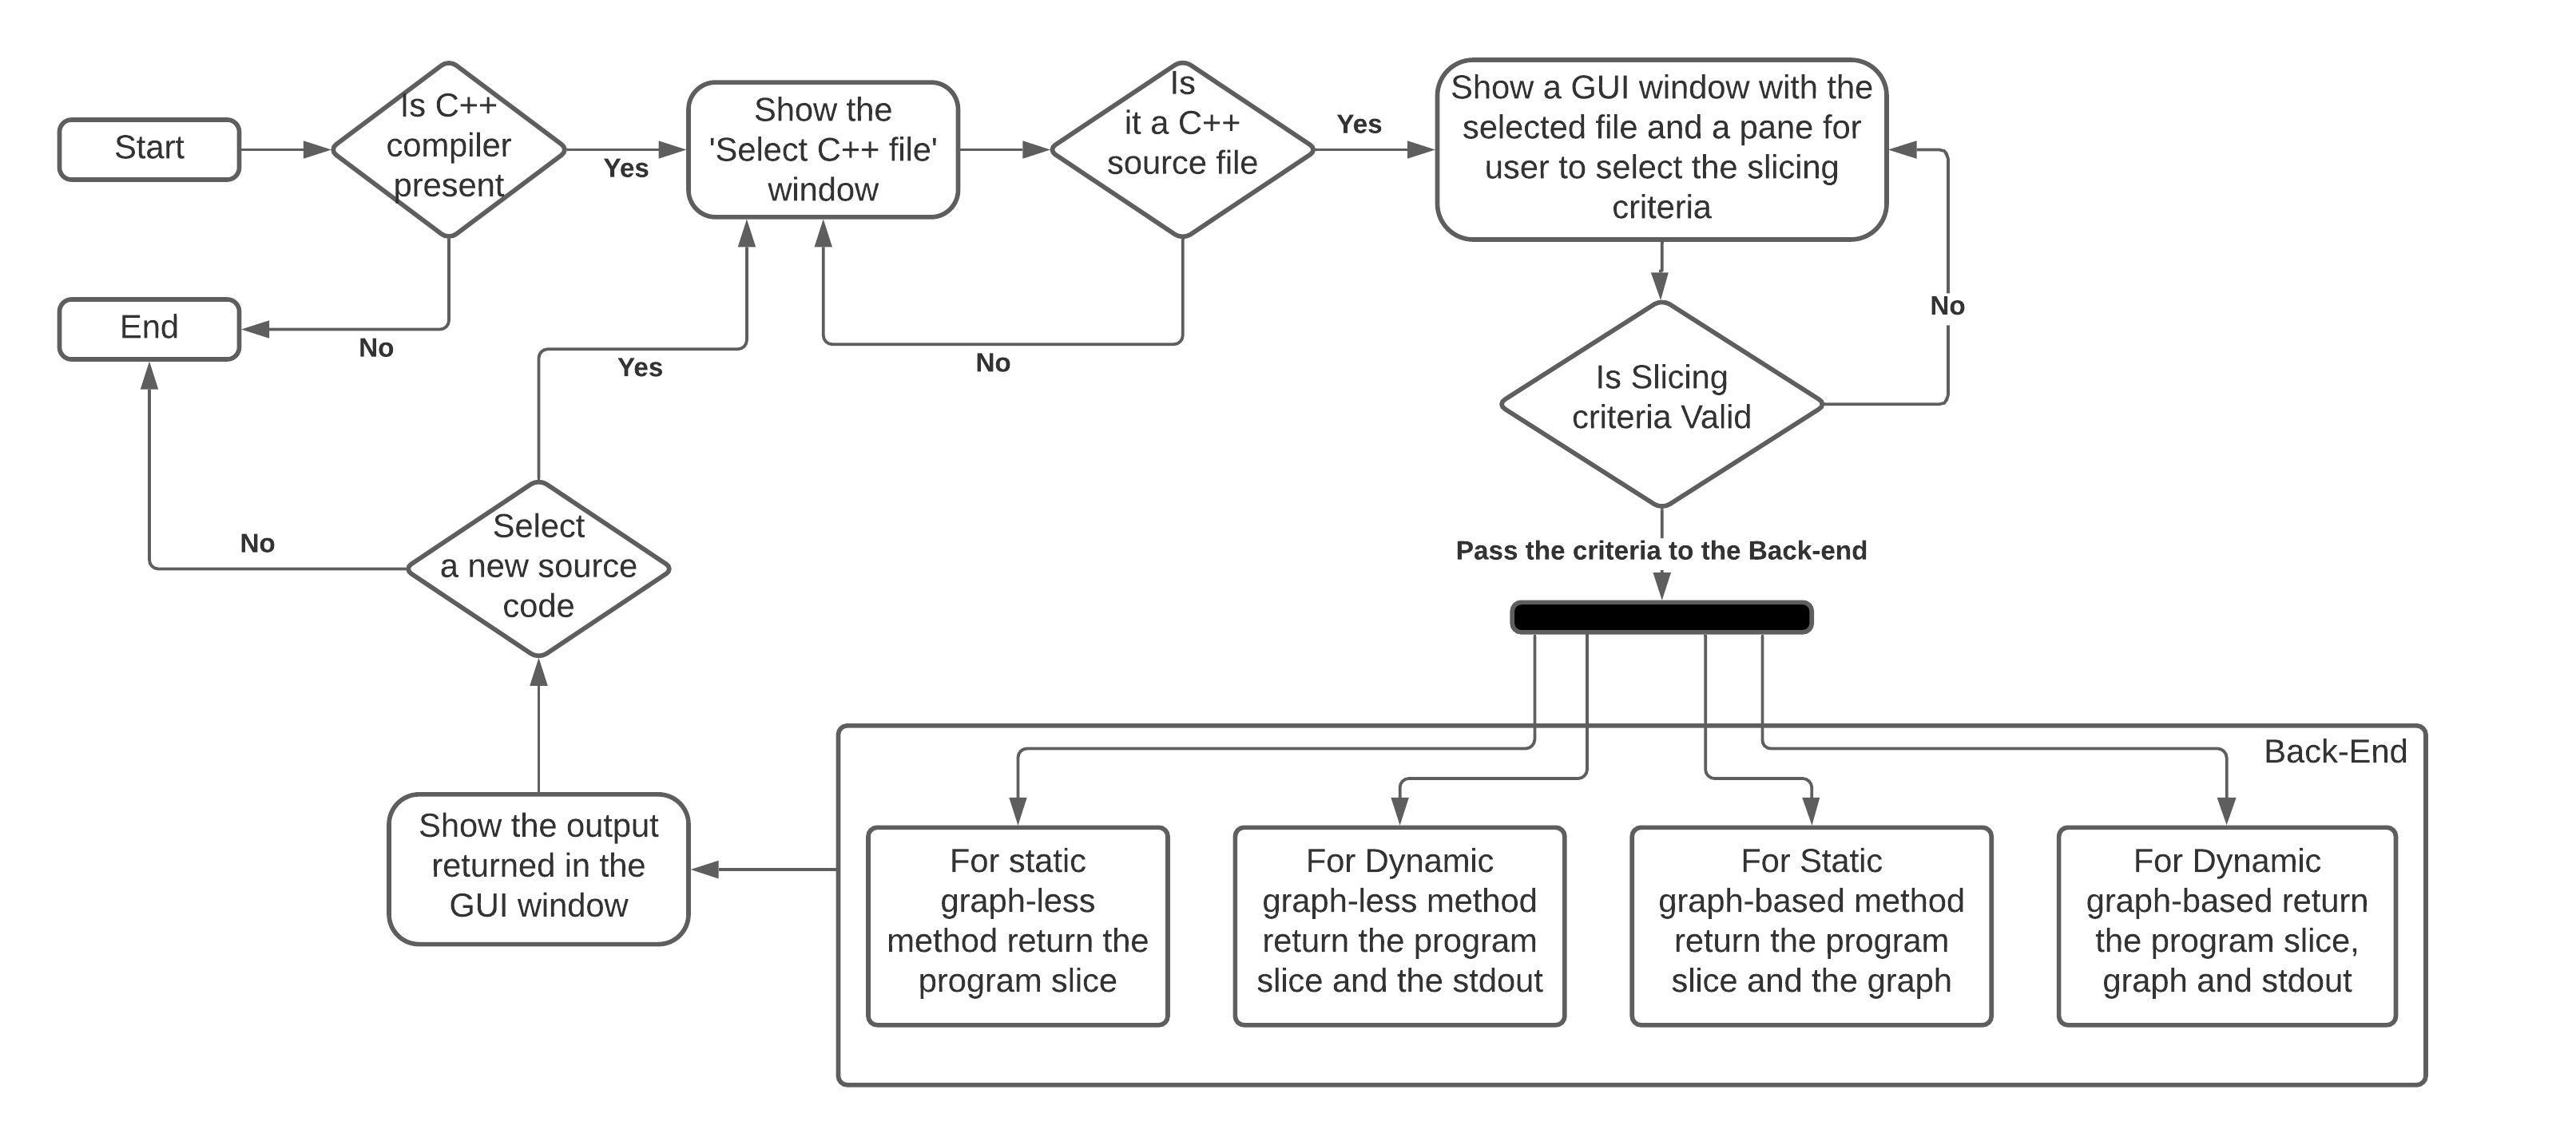
\includegraphics[scale=0.35]{Schematic.jpeg}
    \caption{Schematic diagram showing the implementation flow}
    \label{fig:my_label}
\end{figure}
\subsubsection{Graph-less Slicer}
\par First of all, algorithm checks that is there any external user defined header file is used in the source code or not and add lines from the external user defined header files if used. 
\par In the case of Dynamic Graph-less Slicer, algorithm takes the source code and augment it by adding lines which will help to get the useful information for getting execution trace and memory location of variables at every line. After augmenting source code algorithm executes the updated source code with the help of C++ compiler. Then algorithm starts processing the trace with the firstly executed instruction. Where in the case of the Static Graph-less Slicer, algorithm traverse the source code in two phases. In first phase algorithm traverse the source code and keeps track of scope of user defined functions. So, from second phase on-wards algorithm start parsing source code starting from main functions scope and jumps into different function scope depending upon function call. Algorithm parse the source code and checks if the variable in that line is new or it already exist and if it is new variable than algorithm assigns different unique address. 

\par At each step it computes the dependence set corresponding to the defined variable at the actual instruction, which holds the depending instruction numbers. For this it uses the most recently computed dependence sets of the used variables at the instruction and their last defining instruction. This way all dynamic slices corresponding to the defined variables at all instruction occurrences are attained and provided at the output. Algorithm also keeps track of user defined functions so if source code contains library functions than it can handle it. And at the end algorithm stops parsing source code at the slicing line number provided by the user and returns all the dependent line of the variables provided by user computed up to that line.
\par In case of Static Graph-less Slicer as it does not execute the source code so in case of parallel region, we have assumed that two threads are working on the parallel region in same time and handled slicing accordingly.

\subsubsection{Graph-based Slicer}
\par First of all, Algorithm checks that is there any external user defined header file is used in the source code or not and add lines from the external user defined header files if used. 
\par  In case of Dynamic Graph-based Slicer, algorithm takes the source code and augment it by adding lines which will help to get the execution trace. After augmenting source code algorithm executes the updated source code with the help of C++ compiler. Algorithm start parsing source code starting from first line and according to the instructions it creates nodes and different edges between dependent nodes depending upon different relations. Where in case of Static Graph-based Slicer it does not execute the source code and process all the conditional statements and predicate variables instead of the one which are actually being executed.

\par In case of Static Graph-based Slicer as it does not execute the source code so in case of parallel region, we have assumed that two threads are working on the parallel region in same time and handled slicing accordingly. So the only difference between Dynamic Graph-based Slicer and Static Graph-based Slicer is that static approach does not execute the source code and process all the conditional statements and predicate variables instead of the one which are actually being executed.
\par  Algorithm creates new node for each line. It adds data dependence edge between the nodes where the variable is used to where the variable is last defined before the used variable’s line. It adds control dependence edge between the node and its enclosing scope node. It adds interference dependence edge between nodes where nodes are data dependent to each other but executed from different threads. In case of function call it creates a new node for call site and maintains different nodes known as actual in node for all function arguments, it creates actual out nodes for the function arguments which is passed by reference, it creates formal in nodes at called procedure node for all function parameter, and it creates formal out node for the function parameters which is passed by reference. Transitive dependence edge is created from an actual-in node to an actual-out node if there exist intraslice-path from the formal-out node to formal-in node. For each return site in the called procedure $Q$, a return-link edge is created from the return node in $Q$ to each call site that calls $Q$. If the call site $C$ expects a return value, then the node representing the return value of $C$ in the calling procedure is affect-return dependent on each actual-in node which corresponds to the actual parameter that influences the returned value and is incident to the procedures' call site node. Affect-return dependence is essentially a data dependence much like transitive dependence, except that the return value is never passed into the procedure, so transitive dependence is not appropriate for this situation. It creates parameter-in edge between actual-in and corresponding formal-in node and creates parameter-out edge between formal-out and corresponding actual-out node. It creates calling edge between call site node and called procedure node.

\par After parsing code till slicing line number and creating threaded System dependence graph, algorithm starts slicing on this graph. Algorithm does slice in two passes. This can be done because of the presence of transitive dependence edges, which now include the effect of interference dependencies, at call site. As in sequential slicing, the use of summary information allows the inter-procedural slicer to move across a procedure call without descending into it. The challenges for inter-procedural slicing occur when descending into a called procedure. The context of the call (i.e., the calling procedure) must be maintained. This requires keeping track of the call-order of the procedures during slicing to maintain proper context for ascending back from called procedures. By introducing transitive edges into the tSDG representation, the calling context problem is avoided, as the slicing algorithm can step across a call without descending into it. The slicing problem is still the graph reachability problem. In the first phase of slicing algorithm marks vertices that reach the slicing criterion vertex $s$ and procedure $P$, and are thus in the procedure $P$ itself or a procedure that calls $P$ directly or transitively. Starting at the vertex $s$, algorithm ascends on a certain set of edge types: control dependence, data dependence, interference dependence, parameter-in, transitive dependence, affect-return, and call. During the first phase algorithm never descends into a called procedure, it only ascends. Through the transitive dependence edge that connects actual-out vertices with actual-in vertices, the slicer is able to determine the effects of procedural call without descending into it. The second pass is executed in the same manner as the first pass, but instead of ascending into procedures, it descends into called procedures. Thus, the second pass marks all vertices which reach vertex $s$ from procedures directly or transitively called by $P$, or called directly or transitively by a procedure which directly or transitively calls $P$. As in the sequential algorithm, the first pass must keep track of all call sites encountered as the slicing algorithm ascended, so that it can descend into the procedure at each call site. During the second pass, the following edge types are considered: control dependence, data dependence, interference dependence, parameter-out, transitive dependence, affect-return, and return-link. The second pass is complementary to the first in that it descends into call sites that the first pass skipped. As a last step, the set of vertices from each phase are merged together to get the final set of vertices formed by the slice. And at the end algorithm stops parsing source code at the slicing line number provided by the user and returns all the dependent vertices of the variables provided by user computed up to that line.

\subsection{Handling The OpenMP Constructs}
\begin{itemize}
\item The dynamic and static cases are handled  differently. As we are keeping track of each thread’s thread number in parallel region for each source line execution, so in case of dynamic slicer from that we can get the idea of how many threads are working in that region and in case of static slicer we have assumed that 2 threads are working simultaneously in the parallel region except in cases of sections, single, master constructs exist in the parallel region.
\item On encountering parallel OpenMP construct first of all for all slicers we are finding shared variables so that even after the end of the parallel region we can find it’s definitions. Now in the case of graph-based slicer we have created a hashmap for each thread distinctly to keep track of defined and used variables by different threads. Whereas in case of graph-less slicer we do not need to create a distinct hashmap per thread as we are handling variables by its memory address, so in case of dynamic slicer compiler will create new variable per thread if it is private and in case of static we are doing the same thing manually. And at the end of the parallel region in case of static graph-based and static graph-less slicer we are cloning the whole parallel region for another thread if we haven’t encountered single, master and sections construct.
\item In case of dynamic slicers we can get the information about the threads which have processed these \emph{parallel} control constructs with the help of the compiler as during execution time we have tracked which threads are processing which lines. To handle the for construct in case of static graph-based and static graph-less slicer we have assumed that 2 threads are processing the $for$ loop simultaneously, so after processing those constructs scope once we have cloned whole that scope and then we have found the different relations between these two threads scopes variables. As we know that every section is processed by single threads, so to handle \emph{sections} construct in case of static slicers we increment thread number after completion of each section so that we can fulfill our assumption that each section is processed by different threads. And at the end of sections construct we have found the relation between different variables of different threads. In the case of static slicer single and master constructs are handled by taking root thread to process those scopes.
\item In these algorithms we have handled \emph{private, shared, threadprivate, reduction} data constructs. So the first thing is that we have classified all these data constructs into two categories either shared variables or private variables. Private and shared constructs are self explanatory and categorized into their respective named categories. For the threadprivate construct we have kept those variables in the different hashmap and handled it by considering that if the main thread is processing that variable then we will consider that variable as a shared variable but if other threads are working on it then we have categorized it as a private variable. And for the reduction construct we have considered the reduction variable as a shared variable but everything which is happening on that variable inside of the loop is happening on the private variable. Now after categorizing these constructs we have processed private and shared variables as follows. For that in the case of graph-based approach we have stored shared variables in the hashset. So during the parallel region it is being processed by different threads and according to thread it will be stored in their respective thread’s defined variables and used variables hashmap. But after completing parallel region all the shared variables definitions will be shifted to global defined variables hashmap and after finding the interference dependence between different thread’s variable definitions all these thread's hashmap will be cleared. Whereas in the case of graph-less approach dynamic case is handled automatically by compiler as it gives us a new address for all of the private variables of threads and keeping the same address for shared variables, where for the static case we have mimic the same functionality which compiler does in case of dynamic slicer.
\item On the discovery of the \emph{synchronization} constructs we have handled that by first of all resolving the threads variables means shifting all the shared variables from the threads variable definition hashmap to global variable definition hashmap. Then we have cloned the parallel region till that point in case of static slicers. And after that we have found the relation between variables from the different threads in case of graph-based approach and for the graph-less approach dynamic case is handled automatically due to the presence of compiler where for the static case we have repeated the slicing on the cloned region. 
\end{itemize}
\section{Testing}
Testing can be divided into two parts, one were the algorithms result are tested and in the other part where we test the application which would be used by the user.
\subsection{Testing the Algorithm}
To test the application, we would have to use a sample program, the sample program is as shown below.
\begin{table*}[t]
    \centering
    \begin{tabular}{| p{0.02\textwidth} | p{0.08\textwidth} | p{0.15\textwidth} |p{0.60\textwidth} |p{0.03\textwidth} |}
        \hline
        \textbf{Line No.}&\textbf{Defined}&\textbf{Used}&$Slice$&$LS(d)$\\\hline
    39 & $x$ & $\phi$ & $\phi$ & 39 \\\hline
40 & $y$ & $\phi$ & $\phi$ & 40 \\\hline
41 & $z$ & $\phi$ & $\phi$ & 41 \\\hline
42 & $n$ & $\phi$ & $\phi$ & 42 \\\hline
43 & $k$ & $\phi$ & $\phi$ & 43 \\\hline
44 & $y$ & $\{z\}$ & $\{41\}$ & 44 \\\hline
45 & $x$ & $\{y , z\}$ & $\{41 , 44\}$ & 45 \\\hline
46 & $i$ & $\phi$ & $\{46\}$ & 46 \\\hline
46 & $i$ & $\{i\}$ & $\{46\}$ & 46 \\\hline
46 & $p46(2)$ & $\{n , i\}$ & $\{42 , 46\}$ & 46 \\\hline
6 & $x$ & $\{arg(fun,1)\}$ & $\{41 , 42 , 44 , 45 , 46 , 48\}$ & 6 \\\hline
6 & $y$ & $\{arg(fun,2)\}$ & $\{41 , 42 , 46 , 48\}$ & 6 \\\hline
8 & $k$ & $\phi$ & $\phi$ & 8 \\\hline
9 & $c$ & $\phi$ & $\phi$ & 9 \\\hline
10 & $p10(4)$ & $\phi$ & $\phi$ & 10 \\\hline
12 & $p12(5)$ & $\{y , x , y , p10(4)\}$ & $\{6 , 10 , 41 , 42 , 44 , 45 , 46 , 48\}$ & 12 \\\hline
14 & $k$ & $\{y , x , y , p12(5)\}$ & $\{6 , 10 , 12 , 41 , 42 , 44 , 45 , 46 , 48\}$ & 14 \\\hline
15 & $y$ & $\{y , x , y , p12(5)\}$ & $\{6 , 10 , 12 , 41 , 42 , 44 , 45 , 46 , 48\}$ & 15 \\\hline
17 & $p17(5)$ & $\{y , x , y , p12(5)\}$ & $\{6 , 10 , 12 , 15 , 41 , 42 , 44 , 45 , 46 , 48\}$ & 17 \\\hline
19 & $y$ & $\{y , x , y , p17(5)\}$ & $\{6 , 10 , 12 , 15 , 17 , 41 , 42 , 44 , 45 , 46 , 48\}$ & 19 \\\hline
22 & $p22(4)$ & $\phi$ & $\phi$ & 22 \\\hline
24 & $p24(5)$ & $\{p22(4)\}$ & $\{22\}$ & 24 \\\hline
26 & $i$ & $\{p24(5)\}$ & $\{22 , 24 , 26\}$ & 26 \\\hline
26 & $i$ & $\{i , p24(5)\}$ & $\{22 , 24 , 26\}$ & 26 \\\hline
26 & $p26(6)$ & $\{i , p24(5)\}$ & $\{22 , 24 , 26\}$ & 26 \\\hline
28 & $k$ & $\{i , k , p26(6)\}$ & $\{6 , 10 , 12 , 14 , 15 , 17 , 19 , 22 , 24 , 26 , 41 , 42 , 44 , 45 , 46 , 48\}$ & 28 \\\hline
30 & $x$ & $\{x , k , p24(5)\}$ & $\{6 , 10 , 12 , 14 , 15 , 17 , 19 , 22 , 24 , 26 , 28 , 41 , 42 , 44 , 45 , 46 , 48\}$ & 30 \\\hline
33 & $ret(fun)$ & $\{x\}$ & $\{6 , 10 , 12 , 14 , 15 , 17 , 19 , 22 , 24 , 26 , 28 , 30 , 41 , 42 , 44 , 45 , 46 , 48\}$ & 33 \\\hline
48 & $arg(fun,1)$ & $\{x , p46(2)\}$ & $\{41 , 42 , 44 , 45 , 46\}$ & 48 \\\hline
48 & $arg(fun,2)$ & $\{p46(2)\}$ & $\{42 , 46 \}$ & 48 \\\hline
48 & $x$ & $\{p46(2) , ret(fun)\}$ & $\{6 , 10 , 12 , 14 , 15 , 17 , 19 , 22 , 24 , 26 , 28 , 30 , 33 , 41 , 42 , 44 , 45 , 46 , 48\}$ & 48 \\\hline
49 & $o49$ & $\{i , p46(2)\}$ & $\{42 , 46\}$ & 49 \\\hline
50 & $x$ & $\{x , p46(2)\}$ & $\{6 , 10 , 12 , 14 , 15 , 17 , 19 , 22 , 24 , 26 , 28 , 30 , 33 , 41 , 42 , 44 , 45 , 46 , 48\}$ & 50 \\\hline
52 & $o52$ & $\{x\}$ & $\{6 , 10 , 12 , 14 , 15 , 17 , 19 , 22 , 24 , 26 , 28 , 30 , 33 , 41 , 42 , 44 , 45 , 46 , 48 , 50\}$ & 52 \\\hline
53 & $p53(2)$ & $\{x\}$ & $\{6 , 10 , 12 , 14 , 15 , 17 , 19 , 22 , 24 , 26 , 28 , 30 , 33 , 41 , 42 , 44 , 45 , 46 , 48 , 50\}$ & 53 \\\hline
55 & $y$ & $\{y , p53(2)\}$ & $\{6 , 10 , 12 , 14 , 15 , 17 , 19 , 22 , 24 , 26 , 28 , 30 , 33 , 41 , 42 , 44 , 45 , 46 , 48 , 50 , 53\}$ & 55 \\\hline
56 & $o56$ & $\{y , p53(2)\}$ & $\{6 , 10 , 12 , 14 , 15 , 17 , 19 , 22 , 24 , 26 , 28 , 30 , 33 , 41 , 42 , 44 , 45 , 46 , 48 , 50 , 53 , 55\}$ & 56 \\\hline
58 & $p58(2)$ & $\{x , p53(2)\}$ & $\{6 , 10 , 12 , 14 , 15 , 17 , 19 , 22 , 24 , 26 , 28 , 30 , 33 , 41 , 42 , 44 , 45 , 46 , 48 , 50 , 53\}$ & 58 \\\hline
60 & $x$ & $\{x , k , p58(2)\}$ & $\{6 , 10 , 12 , 14 , 15 , 17 , 19 , 22 , 24 , 26 , 28 , 30 , 33 , 41 , 42 , 43 , 44 , 45 , 46 , 48 , 50 , 53 , 58\}$ & 60 \\\hline
61 & $o61$ & $\{x , p58(2)\}$ & $\{6 , 10 , 12 , 14 , 15 , 17 , 19 , 22 , 24 , 26 , 28 , 30 , 33 , 41 , 42 , 43 , 44 , 45 , 46 , 48 , 50 , 53 , 58 , 60\}$ & 61 \\\hline        
63 & $z$ & $\{x , y\}$ & $\{6 , 10 , 12 , 14 , 15 , 17 , 19 , 22 , 24 , 26 , 28 , 30 , 33 , 41 , 42 , 43 , 44 , 45 , 46 , 48 , 50 , 53 , 55 , 58 , 60\}$ & 63 \\\hline
    \end{tabular}
    \caption{Definition and Use Table(Data Structure) for the Static Method with slicing criterion $<63,z>$}
    \label{tab:my_label}
\end{table*}

\begin{lstlisting}[language=C++]
#include<stdio.h>
#include<conio.h>
#include<iostream>
#include<omp.h>
using namespace std;
int fun(int x, int *y)
{
    int k = 10;
    int c = 10;
    #pragma omp parallel
    {
        if(x > *y) 
        {
            k = x + *y;
            *y = x + *y;
        }
        else if(x < *y)
        {
            *y = x * *y;
        }
    }
    #pragma omp parallel 
    {
        #pragma omp single
        {
            for (int i = 0; i < 2; i = i + 1)
            {
                k = k + i;
            }
            x = x + k;
        }
    }
    return x;
}
int main() 
{
    int x,y,z,n;
    cin>>x;
    cin>>y;
    cin>>z;
    cin>>n;
    int k = 19;
    y = z;
    x = y + z;
    for(int i=0;i<n;i=i+1)
    {
        x = fun(x,&y);
        cout<<i<<endl;
        x = x + 1;
    }
    cout<<x<<endl;
    if(x > 0)
    {
        y = y + 1;
        cout<<y<<endl;
    }
    else if(x < 0)
    {
        x = x + k;
        cout<<x<<endl;
    }
    z = x + y;
}
\end{lstlisting}
 Now we would get the results of the slicing techniques with different slicing criterion, to test the correctness of the algorithms. Now for the present source program the data structure($D/U$ Data structure) used to calculate the slice using the graph-less method would give us the slice shown in $Slice$ and the slice obtained from the algorithm with criteria $<63,z>$ is as below, both are the methods give us same slice, hence the Static Algorithm gives us with the correct slice. To read the $Table$ $II$ and the $Table$ $III$, some terminologies are as follows: 
\begin{itemize}
    \item $LS(d)$ is the line number of the last definition of the variable $d$.
    \item ret($fun$) $\rightarrow$ return statement of 'fun' named function.
    \item p$x$ $\rightarrow$ predicate statements like 'if', 'else', 'for', 'while', where $x$ shows line number.
    \item o$x$ $\rightarrow$ output statements, where $x$ shows line number.
    \item arg($fun$, $x$) $\rightarrow$ function arguments, where first value shows name of the function and second value shows the number of argument.
\end{itemize}
\begin{table*}[t]
    \centering
    \begin{tabular}{| p{0.02\textwidth} | p{0.08\textwidth} | p{0.27\textwidth} |p{0.52\textwidth} |p{0.03\textwidth} |}
        \hline
        \textbf{Line No.}&\textbf{Defined}&\textbf{Used}&$Slice$&$LS(d)$\\\hline
        39 & $x$ & $\phi$ &  $\phi$ & 39\\\hline
        40 & $y$ & $\phi$ &  $\phi$ & 40\\\hline
        41 & $z$ & $\phi$ &  $\phi$ & 41\\\hline
        42 & $n$ & $\phi$ &  $\phi$ & 42\\\hline
        43 & $k$ & $\phi$ &  $\phi$ & 43\\\hline
        44 & $y$ & $\{z\}$ &  $\{41\}$ & 44\\\hline
        45 & $x$ & $\{y , z\}$ &  $\{41 , 44\}$ & 45\\\hline
        46 & $i$ & $\phi$ &  $\phi$ & 46\\\hline
        46 & $p46(2)$ & $\{i , n \}$ &  $\{42 , 46\}$ & 46\\\hline
        48 & $arg(fun,1)$ & $\{x , p46(2)\}$ &  $\{41 , 42 , 44 , 45 , 46\}$ & 48\\\hline
        48 & $arg(fun,2)$ & $\{p46(2)\}$ &  $\{42 , 46 , \}$ & 48\\\hline
        6 & $x$ & $\{arg(fun,1)\}$ &  $\{41 , 42 , 44 , 45 , 46 , 48\}$ & 6\\\hline
        6 & $y$ & $\{arg(fun,2)\}$ &  $\{41 , 42 , 46 , 48\}$ & 6\\\hline
        8 & $k$ & \phi &  \phi & 8\\\hline
        9 & $c$ & \phi &  \phi & 9\\\hline
        12 & $p12(6)$ & $\{y, \textit{\#pragma omp parallel\#10}\}$ &  $\{6 , 10 , 41 , 42 , 46 , 48 \}$ & 12\\\hline
        14 & $k$ & $\{x , y , p12(6)\}$ &  $\{ 6 , 10 , 12 , 41 , 42 , 44 , 45 , 46 , 48\}$ & 14\\\hline
        15 & $y$ & $\{x , y , p12(6)\}$ &  $\{ 6 , 10 , 12 , 41 , 42 , 44 , 45 , 46 , 48\}$ & 15\\\hline
        12 & $p12(5)$ & $\{y , \textit{\#pragma omp parallel\#10 }\}$ &  $\{6 , 10 , 12 , 15 , 41 , 42 , 44 , 45 , 46 , 48\}$ & 12\\\hline
        17 & $p17(5)$ & $\{ y , p12(5) ,\textit{\#pragma omp parallel\#10(5)}\}$ &  $\{ 6 , 10 , 12 , 15 , 41 , 42 , 44 , 45 , 46 , 48\}$ & 17\\\hline
        19 & $y$ & $\{x , y , p17(5)\}$ &  $\{6 , 10 , 12 , 15 , 17 , 41 , 42 , 44 , 45 , 46 , 48\}$ & 19\\\hline
        12 & $p12(5)$ & $\{y , \textit{\#pragma omp parallel#10}\}$ &  $\{ 6 , 10 , 12 , 15 , 17 , 19 , 41 , 42 , 44 , 45 , 46 , 48 \}$ & 12\\\hline
        17 & $p17(5)$ & $\{y , p12(5) , \textit{\#pragma omp parallel\#10(5)}\}$ &  $\{6 , 10 , 12 , 15 , 17 , 19 , 41 , 42 , 44 , 45 , 46 , 48 \}$ & 17\\\hline
        19 & $y$ & $\{x , y , p17(5)\}$ &  $\{ 6 , 10 , 12 , 15 , 17 , 19 , 41 , 42 , 44 , 45 , 46 , 48\}$ & 19\\\hline
        12 & $p12(5)$ & $\{y, \textit{\#pragma omp parallel\#10}\}$ &  $\{ 6 , 10 , 12 , 15 , 17 , 19 , 41 , 42 , 44 , 45 , 46 , 48\}$ & 12\\\hline
        17 & $p17(5)$ & $\{y ,p12(5) ,\textit{\#pragma omp parallel\#10(5)} \}$ &  $\{6 , 10 , 12 , 15 , 17 , 19 , 41 , 42 , 44 , 45 , 46 , 48\}$ & 17\\\hline
        19 & $y$ & $\{x , y , p17(5)\}$ &  $\{6 , 10 , 12 , 15 , 17 , 19 , 41 , 42 , 44 , 45 , 46 , 48\}$ & 19\\\hline
        26 & $i$ & $\{\textit{\#pragma omp single\#24}\}$ &  $\{22 , 24\}$ & 26\\\hline
        26 & $p26(9)$ & $\{i ,\textit{\#pragma omp single\#24}\}$ &  $\{22 , 24 , 26\}$ & 26\\\hline
        28 & $k$ & $\{k , i , p26(9)\}$ &  $\{6 , 10 , 12 , 14 , 22 , 24 , 26 , 41 , 42 , 44 , 45 , 46 , 48\}$ & 28\\\hline
        26 & $i$ & $\{i ,\textit{\#pragma omp single\#24}\}$ &  $\{22 , 24 , 26 \}$ & 26\\\hline
        26 & $p26(9)$ & $\{i , \textit{\#pragma omp single\#24}\}$ &  $\{22 , 24 , 26 \}$ & 26\\\hline
        28 & $k$ & $\{k , i , p26(9)\}$ & $\{6 , 10 , 12 , 14 , 22 , 24 , 26 , 28 , 41 , 42 , 44 , 45 , 46 , 48\}$ & 28 \\\hline
        30 & $x$ & $\{x , k , \textit{\#pragma omp single\#24}\}$ & $\{6 , 10 , 12 , 14 , 22 , 24 , 26 , 28 , 41 , 42 , 44 , 45 , 46 , 48\}$ & 30 \\\hline
        33 & $ret(fun)$ & $\{x\}$ & $\{6 , 10 , 12 , 14 , 22 , 24 , 26 , 28 , 30 , 41 , 42 , 44 , 45 , 46 , 48\}$ & 33 \\\hline
        48 & $x$ & $\{ret(fun) , p46(2)\}$ & $\{6 , 10 , 12 , 14 , 22 , 24 , 26 , 28 , 30 , 33 , 41 , 42 , 44 , 45 , 46 , 48\}$ & 48 \\\hline
        49 & $o49$ & $\{i , p46(2)\}$ & $\{42 , 46\}$ & 49 \\\hline
        50 & $x$ & $\{x , p46(2)\}$ & $\{6 , 10 , 12 , 14 , 22 , 24 , 26 , 28 , 30 , 33 , 41 , 42 , 44 , 45 , 46 , 48\}$ & 50 \\\hline
        52 & $o52$ & $\{x\}$ & $\{6 , 10 , 12 , 14 , 22 , 24 , 26 , 28 , 30 , 33 , 41 , 42 , 44 , 45 , 46 , 48 , 50\}$ & 52 \\\hline
        53 & $p53(2)$ & $\{x\}$ &  $\phi$ & 53 \\\hline
        55 & $y$ & $\{y , p53(2)\}$ &  $\{6 , 10 , 12 , 15 , 17 , 19 , 41 , 42 , 44 , 45 , 46 , 48 , 53\}$ & 55 \\\hline
        56 & $o56$ & $\{y , p53(2)\}$ &  $\{6 , 10 , 12 , 15 , 17 , 19 , 41 , 42 , 44 , 45 , 46 , 48 , 53 , 55\}$ & 56 \\\hline
        63 & $z$ & $\{x , y\}$ & $\{6 , 10 , 12 , 14 , 15 , 17 , 19 , 22 , 24 , 26 , 28 , 30 , 33 , 41 , 42 , 44 , 45 , 46 , 48 , 50 , 53 , 55\}$ & 63 \\\hline
    \end{tabular}
    \caption{Definition and Use Table(Data Structure) for the Dynamic Method with slicing criterion $<,63,z,\{1,2,3,1\}>$}
    \label{tab:my_label}
\end{table*}
\begin{lstlisting}
6 : int fun(int x, int *y)
10 :     #pragma omp parallel
12 :         if(x > *y) 
14 :             k = x + *y;
15 :             *y = x + *y;
17 :         else if(x < *y)
19 :             *y = x * *y;
22 :     #pragma omp parallel 
24 :         #pragma omp single
26 :             for (int i = 0; i < 2; i = i + 1)
28 :                 k = k + i;
30 :             x = x + k;
33 :     return x;
41 :     cin>>z;
42 :     cin>>n;
43 :     int k = 19;
44 :     y = z;
45 :     x = y + z;
46 :     for(int i=0;i<n;i=i+1)
48 :         x = fun(x,&y);
50 :         x = x + 1;
53 :     if(x > 0)
55 :         y = y + 1;
58 :     else if(x < 0)
60 :         x = x + k;
63 :     z = x + y;
\end{lstlisting}
\begin{figure*}[p]
    \centering
    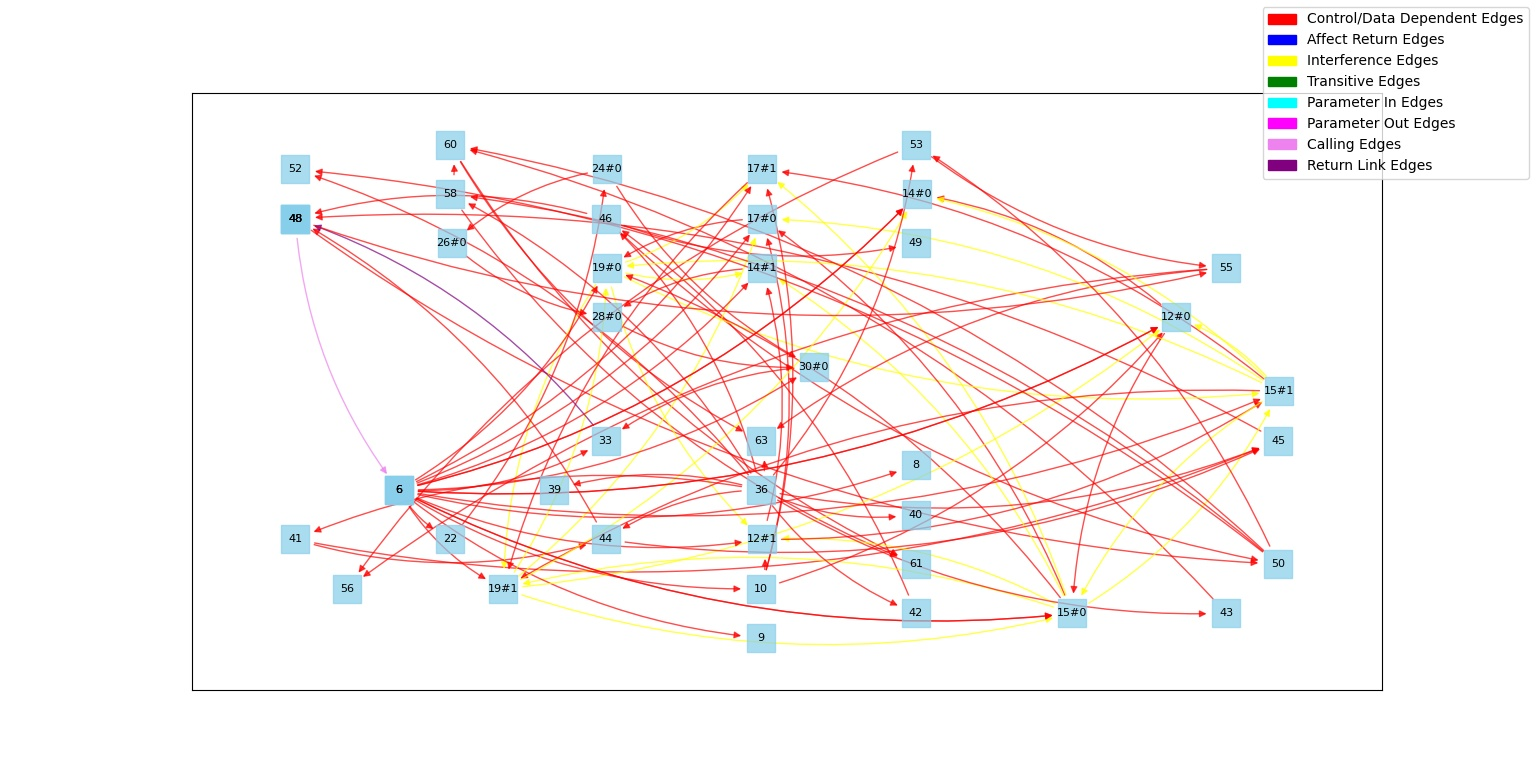
\includegraphics[scale=0.5]{sourcetSDG.jpeg}
    \caption{Source Program tSDG}
    \label{fig:my_label}
\end{figure*}
\begin{figure*}[p]
    \centering
    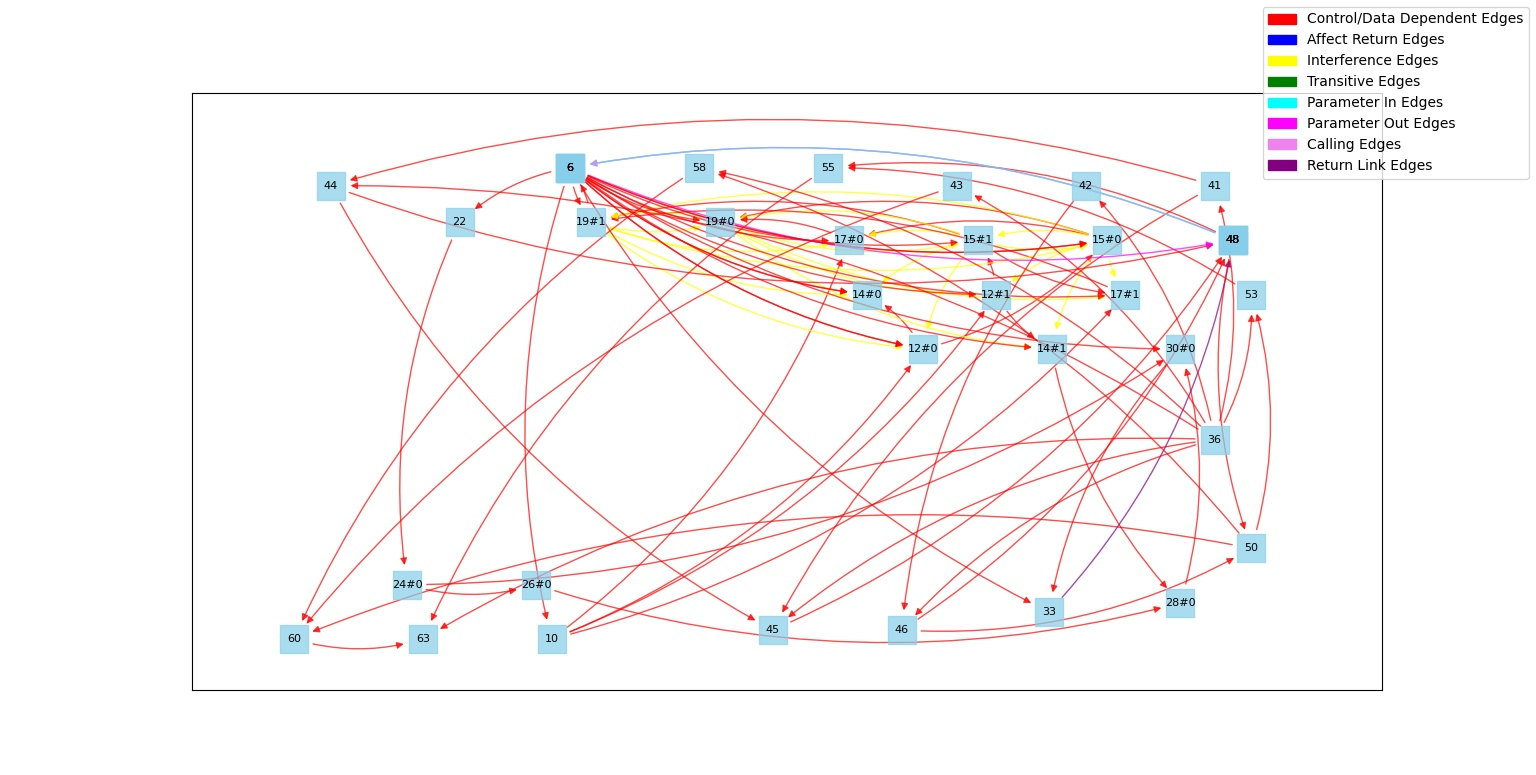
\includegraphics[scale=0.5]{sourceSGz.jpeg}
    \caption{Static Graph Method's generated graph with the slicing criterion $<63,z>$}
    \label{fig:my_label}
\end{figure*}
\begin{figure*}[t]
    \centering
    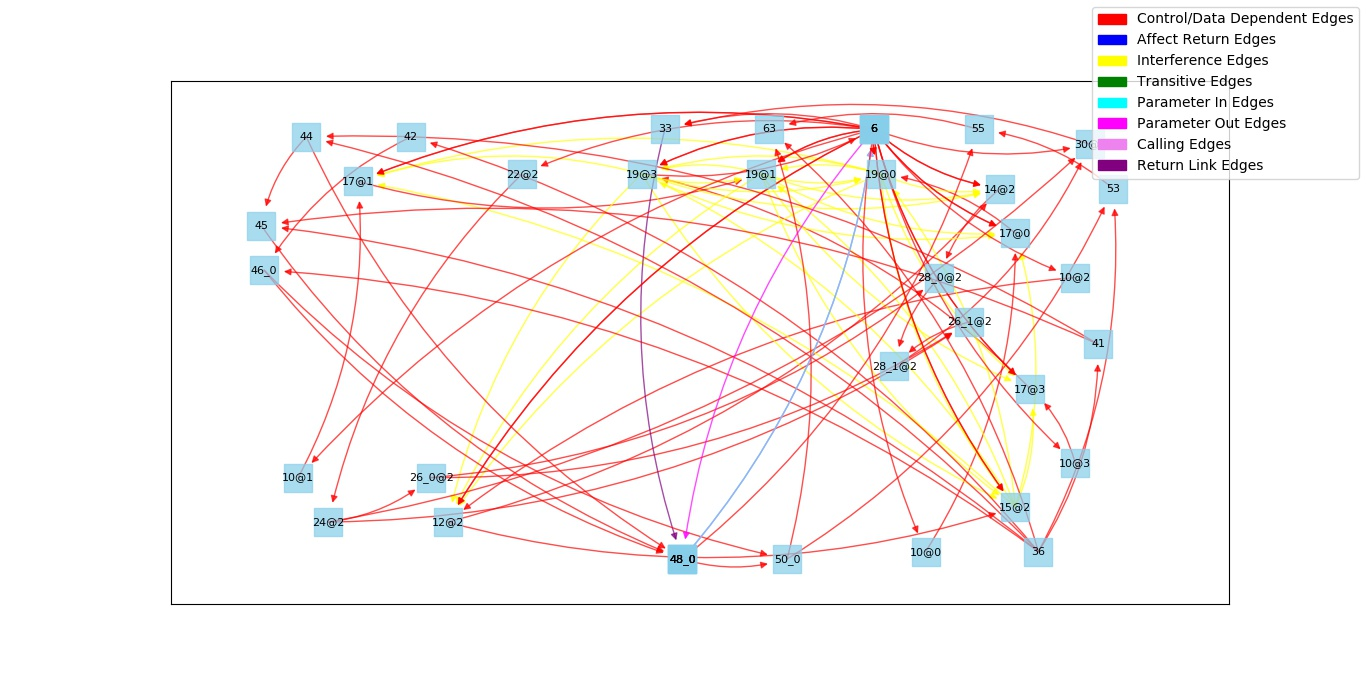
\includegraphics[scale=0.5]{sourceDG.jpeg}
    \caption{Dynamic Graph Method's generated graph with the slicing criterion $<,63,z,\{1,2,3,1\}>$}
    \label{fig:my_label}
\end{figure*}

Now, in the case of the Dynamic Graph-less method, where we would have to give a input to the program, in this case the input is $<1,2,3,1>$. The $D/U$ Table is as shown in the $Table$ $III$ and the slice obtained from the algorithmic method is as shown below and both the methods give the same slice.
\begin{lstlisting}
6 : int fun(int x, int *y)
8 :     int k = 10;
10 :     #pragma omp parallel
12 :         if(x > *y) 
14 :             k = x + *y;
15 :             *y = x + *y;
17 :         else if(x < *y)
19 :             *y = x * *y;
22 :     #pragma omp parallel 
24 :         #pragma omp single
26 :             for (int i = 0; i < 2; i = i + 1)
28 :                 k = k + i;
30 :             x = x + k;
33 :     return x;
41 :     cin>>z;
42 :     cin>>n;
43 :     int k = 19;
44 :     y = z;
45 :     x = y + z;
46 :     for(int i=0;i<n;i=i+1)
48 :         x = fun(x,&y);
50 :         x = x + 1;
53 :     if(x > 0)
55 :         y = y + 1;
63 :     z = x + y;
\end{lstlisting}
As shown in $Fig.$ 3, what we can see is the Source Program's tSDG, Now the slices that we will obtain from the graph based methods must be the sub-graph of this graph. $Fig.$ $4$ shows the graph that we obtained as the output using the static graph-based method using the criteria $<63,z>$. Now the slice that we want from the method is as below, the slice below are all the nodes that should be present in the graph generated by the static graph-based method. Both the slices have the same nodes present in them, hence the slice obtained from the method is correct.  
% Static graphbase :z
\begin{lstlisting}
6 : int fun(int x, int *y)
6 : y_out = *y
6 : y = y_in
6 : x = x_in
10 :    #pragma omp parallel
12#0 :        if(x > *y) 
12#1 :        if(x > *y) 
14#0 :            k = x + *y;
14#1 :            k = x + *y;
15#0 :            *y = x + *y;
15#1 :            *y = x + *y;
17#0 :        else if(x < *y)
17#1 :        else if(x < *y)
19#0 :            *y = x * *y;
19#1 :            *y = x * *y;
22 :    #pragma omp parallel 
24#0 :        #pragma omp single
26#0 :            for (int i = 0; i < 2; i = i + 1)
28#0 :                k = k + i;
30#0 :            x = x + k;
33 :    return x;
36 : int main() 
41 :    cin>>z;
42 :    cin>>n;
43 :    int k = 19;
44 :    y = z;
45 :    x = y + z;
46 :    for(int i=0;i<n;i=i+1)
48 :        x_in = x
48 :        y = &y_out
48 :        x = fun(x,&y);
48 :        y_in = y
50 :        x = x + 1;
53 :    if(x > 0)
55 :        y = y + 1;
58 :    else if(x < 0)
60 :        x = x + k;
63 :    z = x + y;
\end{lstlisting}
In the case of Dynamic Graph-based method, the graph that the algorithm's implementation gave is as shown in $Fig.$ $5$. The slice that we want to obtain from the graph must have the nodes as shown in the method's slice as shown below. In this case too, both the representations have the same node, implying that the slices generated are the same.

\begin{table*}[t]
\begin{center}
\begin{tabular}{| p{0.40\textwidth} | p{0.30\textwidth} | p{0.30\textwidth} |}
\hline
    \textbf{Test Case Description} & \textbf{Expected Result} & \textbf{Test Result}  \\
\hline
    Select a file from the 'Select file' Dialog box when user clicks on 'Select File' button. & find the file location in the variable storing the selected file. & the file location was found at the wanted location. \\
\hline
    Compile the selected file and see if the interface can check the compilation status of the file. & A executable created if there are no compilation errors in the source file or a warning to the user in case of any errors. & The executable was found at the wanted location and a warning appeared displaying the compilation errors in case of a faulty C++ file. \\
\hline
    Compile the Algorithm files that are in the same folder as the application file. & find the executable files of all the algorithm files needed for execution of algorithm. & Found the executable files at the desired location.  \\
\hline
    Execute an algorithm with a C++ file with OpenMP constructs to find the slice of the program. & Find a generated slice file and also the module reading the slice to display the slice to the user. & Found the required file and also the module was able to process the file to the desired outcome.\\
\hline
    In case of a method that generates graph as an output, some files that save the required data to generate the graphs would be needed for graph generation module. & The graph files should be found after execution and also the graph files can be accessed by the graph generation module. & The required files were at the location and the module was  able to access the desired resources.\\
\hline
    Test the module which is called at the time of closing the application to delete all the generated temporary files by the application. & Not find any temporary files after the closing of the application. & Failed to find an temporary generated files by the application.\\
\hline
\end{tabular}
\end{center}
\caption{Test Case Results}
\label{tab:template}
\end{table*}


% Dynamic Graphbase: z input(1,2,3,1)
\begin{lstlisting}
6 : int fun(int x, int *y)
6 : y_out = *y
6 : x = x_in
6 : y = y_in
10@0 :    #pragma omp parallel
10@1 :    #pragma omp parallel
10@2 :    #pragma omp parallel
10@3 :    #pragma omp parallel
12@2 :        if(x > *y) 
14@2 :            k = x + *y;
15@2 :            *y = x + *y;
17@0 :        else if(x < *y)
17@1 :        else if(x < *y)
17@3 :        else if(x < *y)
19@0 :            *y = x * *y;
19@1 :            *y = x * *y;
19@3 :            *y = x * *y;
22@2 :    #pragma omp parallel 
24@2 :        #pragma omp single
26_0@2 :            for (int i = 0; i < 2; i = i + 1)
26_1@2 :            for (int i = 0; i < 2; i = i + 1)
28_0@2 :                k = k + i;
28_1@2 :                k = k + i;
30@2 :            x = x + k;
33 :    return x;
36 :int main() 
41 :    cin>>z;
42 :    cin>>n;
44 :    y = z;
45 :    x = y + z;
46_0 :    for(int i=0;i<n;i=i+1)
48_0 :        y = &y_out
48_0 :        y_in = y
48_0 :        x_in = x
48_0 :        x = fun(x,&y);
50_0 :        x = x + 1;
53 :    if(x > 0)
55 :        y = y + 1;
63 :    z = x + y;
\end{lstlisting}

The tests were also done for different slicing criterion like $<45,x,\{-1,2,3,1\}>$ and $<56,y,\{47,100,30,11\}>$, but the results were only presented for one of the criteria. Now, if we compare the graph-based and graph-less techniques, we can see one thing both use different ways to obtain the slices, one the $tSDG$ and other $D/U$ table, but the corresponding static slices and also the dynamic slices are same for the same slicing criteria. The only difference is in the time and memory complexity. Graph-less algorithm consumes less time and memory compare to graph-base algorithms. So, in this section we presented a view of how the black-box testing of algorithm's implementation was carried out. 

\subsection{Testing Application}

The testing strategy for the developed application with the individual components was do the perform the tests after doing the code reviews for each of the components. Now instead of having user files, for the purpose of the testing , some predefined C++ OpenMP codes were used which would have the constructs that are supported by the application. 
\par First to test the individual components, Unit testing was performed using the Python's \emph{unittest} library . The test cases were designed to test the modules and if the modules provided the required function that was needed. The test cases used Mock Objects to test the modules, where needed as the focus here is more on the potential bugs that may be present in the individual modules. Some test cases used the black box testing where focus was more on if the output generated was expected or not for the given input and other test cases used the Gray box testing technique where the given tested module's functional behaviour was also tested.
\par To test the integration between the different modules, was to test for if the communication between them is as expected, and try to find different scenarios that would possibly affect them. The technique here used was the bottom-up incremental testing, where we tried to go through the tests in such a way that at the end of all tests, all the logically related components were tested. The table here shows the tests and if the expected results were found or not.

\par After completing the Unit and Integration testing, the focus on the performance aspect. A module was created to record all the performance metrics  that are important like the parameters related to the speed(execution time), the scalability parameters(source code line count, the output slice line count) and the algorithm that was selected by the user. The records that are saved show that the 'graph' method for the same counterpart takes more time than the 'non-graph' method, as the module related to generate graph accounts for that increased time. The test results also show that the 'Dynamic' methods are taking more time than the 'Static' methods. 

\section{Conclusion}
\par This project tried to use the algorithms that were available and to update the algorithm so that finding the program slice of Shared memory parallel programs. To visualize the results of the algorithm using the graphs and in case of non-graph based methods using the data structures.Then the objective was to develop an interface such that an user could use the algorithms on the user given programs. 

\par The Future work of the current project, would be improve the parser such that it can parse more C++ statements. Also improve the algorithms such that it can handle more OpenMP constructs, so they can be represented in the algorithms and their role in slice can  be known. Also, improvement in the scale of programs that can be handled needs to be improved. One important that can also be added is implementing the algorithms such that user can interact with the algorithms like an API. 

\section{Related Works}
\par Plenty of work has already been done in the field of program slicing. 
Ferrante $et$ $al.$\cite{b7}  had first proposed the representation technique named Program Dependence Graph (PDG). To overcome the shortcomings of PDG, Horwitz $et$ $al.$\cite{b8} proposed an extended version of PDG known as System Dependence Graph (SDG) which helps to find inter-procedural static program slices under the same graph reachability framework. As SDG is basically a collection of the different sub-routine's PDG.  Livadas $et$ $al.$\cite{b9} proposed another better approach for the computation of inter-procedural slices, By creating the SDG in the bottom-up manner and by descending into the called procedure to process them first if that particular procedure is not yet processed. If that procedure is already being processed then just reflect that summary information at the calling point. In this paper, we have followed this approach for the construction of the graph-based slicer where we have used $tSDG$. 

\par Korel $et$ $al.$\cite{b10} developed algorithms for the dynamic case by extending the static slicing algorithms. They defined the dynamic slice in such a way that would include all the occurrences of a particular statement in the slice if any one occurrence of a statement in the execution history $EH$ is included in the slice, even when the value of the variable in question at the given location is unaffected by the other occurrences. So the dynamic slice obtained is executable and produces the same value of the variable in question at the given location as the original program but it generates a very large unnecessary dynamic slice. But here our purpose is not to generate a slice which is executable but which gives an accurate and compact slice so we have considered only those lines which actually affects the value of that variable. Korel and Yalamanchili\cite{b11} developed a forward computation method, for the graph-less slicing methods.

\section*{Acknowledgment}
This project would not have been possible without the guidance and mentorship of prof. Jayprakash Lalchandani. We would also like to thank our family members, friends and the colleagues who helped us throughout the project. We are also grateful to Dhirubhai Institute of Information and Communication Technology, which provided us the important knowledge and opportunity to carry out this project.


\section*{Appendix}
\subsection{Parallel Control Constructs}
As OpenMP uses fork-join model, basically \emph{PARALLEL} construct basically creates threads to execute a section enclosed by the construct. \emph{FOR} construct is to explicitly parallelize loop control structures in the enclosed section. \emph{SECTIONS} constructs is to create threads to execute each \emph{SECTION} construct enclosed on a separate thread. \emph{SINGLE} construct would only one thread to execute the section if there are multiple threads created for the task and similarly \emph{MASTER} construct only allows the master thread to execute the task. So, this constructs are basically which are used to do the work-sharing among threads by creating them.
\subsection{Data Constructs}
These constructs are basically used to handle the data race conditions where each thread might affect the data individually and if it isn't handled properly, the program may give unwanted results. \emph{THREADPRIVATE} would generate for each thread their own copy of the variable, \emph{PRIVATE} is used to declare the list of variables only available to the tasks that are enclosed and on the contrary \emph{SHARED} declares the list of variables to be shared among the tasks. \emph{REDUCTION} basically shares the variables to each thread by giving them their own copy but at the end get the results into the original variable with the specified identifier.
\subsection{Synchronization Constructs}
These constructs basically convert the section enclosed into a sequential block of code and to be executed only by a thread so there are no synchronization problems. \emph{CRITICAL} would only allow one thread to execute the enclosed block. \emph{BARRIER} creates an explicit barrier such that all threads much reach the point. \emoh{FLUSH} is used to make the thread's view of the primary memory similar to that of the main memory.
\subsection{Basic Block}
\par A basic block is nothing but a consecutive sequence of instructions that has a single entry point and a single exit point. In this algorithm, we have considered only one instruction per block. This allows more accurate slices to be calculated as dependence between blocks becomes dependence between single instructions and not multiple instructions.
\subsection{Control Flow Graph} 
CFG represents a program with the help of execution order of program. So basically, it will create a node for each basic block (which contains single instruction) and adds the control flow edge between two nodes if there exist possible execution path from one node to another. 
\subsection{Program Dependence Graph}
\par PDG of the program is a directed graph in which nodes represents predicates and statements and edges represents data and control dependence among the nodes.
\subsection{System Dependence Graph}
\par SDG is basically a group of PDGs. So actually, what happens is SDG will generate different PDG for different procedures and connects all of these PDGs with the help of different nodes and edges at calling location. 
\subsection{tPDG and tSDG}
\par The only difference between PDG, SDG and tPDG, tSDG respectively is that tPDG and tSDG includes one extra edge called interference edge apart from the other edges added in PDG and SDG. 
\begin{thebibliography}{00}
\bibitem{b1} 
F. Tip: A survey of program slicing techniques.\\
\emph{Journal of Programming Languages}, 3(3):121–189, Sept. 1995.
\bibitem{b2} 
A. Beszedes, T. Gergely, Zs. M. Szabo, J. Csirik, and
T. Gyimothy: Dynamic slicing method for maintenance of
large C programs.\\
In\emph{ Proceedings of the Fifth European
Conference on Software Maintenance and Reengineering
(CSMR 2001)}, pages 105–113. Mar. 2001.
\bibitem{b3}
A. Beszedes, T. Gergely, Zs. M. Szabo, J. Csirik, and
T. Gyimothy: Graph-Less Dynamic Dependence-Based Dynamic Slicing Algorithms.
\bibitem{b4} 
H. Agrawal and J. Horgan: Dynamic program slicing.\\
In \emph{SIGPLAN Notices No. 6}, pages 246–256, 1990.
\bibitem{b5}
D. Hisley, M. Bridges and L. Pollock :Static Interprocedural Slicing of Shared Memory Parallel Programs
\bibitem{b6}
 M. Bridges :Program Slicing Of Explicitly Parallel Programs\\
Thesis submitted to \emph{Faculty of University of Delaware}, 2002. 
\bibitem{b7}
Jeanne Ferrante, Karl Ottenstein, and Joe Warren: The program dependence graph and its uses in optimization.\\
\emph{ACM Transactions on Programming Languages and Systems}, July 1987.
\bibitem{b8}
Susan Horwitz, Thomas Reps and David Binkeley: Inter-procedural slicing using dependence graphs. 
\emph{ACM SIGPLAN'88 Conference on Programming Language Design and Implementation}, 1988.
\bibitem{b9}
P. Livadas and S. Croll: A new algorithm for the calculation of transitive dependencies.
\emph{Journal of Software Maintenance}, 1994.
\bibitem{b10}
Bogdan Korel and Janusz Laski: Dynamic program slicing. 
\emph{Information Processing Letters}, 1988.
\bibitem{b11}
B. Korel and S. Yalamanchili: Forward computation of dynamic program slices. 
In Proceedings of \emph{1994 International Symposium on Software Testing and Analysis (ISSTA)}, 1994.

\end{thebibliography}


 \end{document}